\documentclass{article}

% Language setting
% Replace `english' with e.g. `spanish' to change the document language
\usepackage[spanish]{babel}

% Set page size and margins
% Replace `letterpaper' with `a4paper' for UK/EU standard size
\usepackage[letterpaper,top=2cm,bottom=2cm,left=3cm,right=3cm,marginparwidth=1.75cm]{geometry}

% Useful packages
\usepackage{amsmath}
\usepackage{graphicx}
\usepackage[colorlinks=true, allcolors=blue]{hyperref}
\ProvidesPackage{whilecode2}
\RequirePackage{listings}
\RequirePackage{suffix}
\RequirePackage[onelanguage, linesnumbered, noline, resetcount]{algorithm2e}

\title{Práctica 3 TALF}
\author{Omar Lukach Temsamani}

\begin{document}
\maketitle

\section{Ejercicio 1}
\subsection{Enunciado}
Una imagen de la Máquina de Turing definida con JFLAP:
\\
Define the TM solution of exercise 3.4 of the problem list and test its correct
behaviour.

\subsection{Imagen de la máquina en JFLAP}

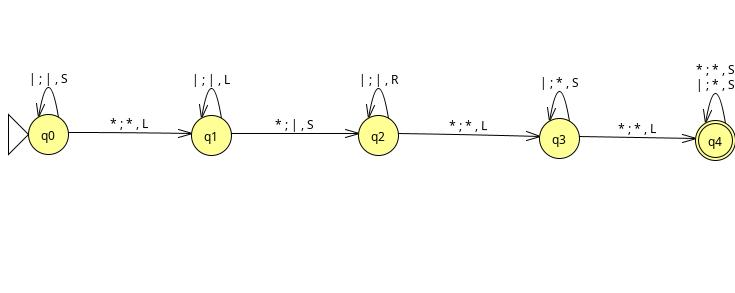
\includegraphics[width=0.8\textwidth]{p3ej1.jpg}

\section{Ejercicio 3}

\subsection{Enunciado}
Implement a WHILE program that computes the sum of three values. You
must use an auxiliary variable that accumulates the result of the sum.

\subsection{Resolución}
\newenvironment{whilecode}
\begin{whilecode}
  $X_1 := X_1 + X_2$\;
  $X_1 := X_1 + X_3$\;
  $X_1 := X_1 + X_4$\;


\end{document}